%Writeup for ENGR202 Lab {INSERT LAB #}
%If editing in vim/vi please insert your own line breaks! This will help keep the file cleaner and easier to edit.

%::Collaboration etiquette::
%In order to better identify changes
%please surround all edits with your
%name as follows:

%BEGIN Zach
%END Zach

%LaTeX will ignore line breaks so to denote
%changes in the middle of a line begin the
%edits on a new line after your name tag
%and then continue with the original on
%the next line following your ending name
%tag.



\documentclass{article}
\usepackage{graphicx}
\graphicspath{ {images/} }

%Change # to correct lab number!
\title{\textbf{Chapter 4 Lab Writeup}}
\author{Zach Thompson, Simon Hannes, Kyle Peterson}
\begin{document}

\maketitle{}

\section*{Overview}
%BEGIN SIMON
\paragraph{}
The purpose of this lab is to determine which components are within the Mystery
Boxes.The first box examined contained one component while the second contained
two components in series. 
%END SIMON

\section*{Process}
%BEGIN SIMON
\paragraph{}
To determine the content of the boxes, we connected a 1k resistor in series
to the boxes, applied a DC voltage to the box and resistor, and measured the
result. We noted the voltage response across the resistor and across the box.
As expected, the sum of these two voltages was equal to the voltage applied.
We then divided the voltage drop across the resistor by the known value of
the resistor to determine current. All components are in series, and thus the
current through the resistor is equal to the current through the box. Impedence
of the box can then be determined by dividing voltage drop across the box by
the current of the circuit. We then applied an AC current at five different
frequencies and determined the phase difference of the resultant voltage drop
vs the original applied voltage. We varied the frequency to produce an
approximately $\angle{}45^\circ{}$ difference.
%END SIMON

\section*{Results}
%BEGIN SIMON
\paragraph{}
Here are the numerical results we found for each respective box.

\subsection*{Box: Mercedes Benz}
\paragraph{}
We began by testing the resistor for accuracy using the multimeter and found
it to be $979\Omega{}$. We also tested the box alone for resisitivity and found
a very small value, suggesting an inductor. We connected a $5V$ DC power supply
to the resistor and box in series, and set the multimeter to voltage mode. We
found a $4.8V$ drop across the resistor and a $115mV$ drop across the box. Next,
we connected a $5V$ AC source at $1KHz$ cooresponding to a source sinusoid of
$5\cos{}(2000\pi{} t)$. The time delay between the source voltage and voltage 
measured across the box was found to be $190\mu{} s$.The phase shift is then 
given by: $\angle{} = 360^\circ{}(1000Hz)(190\mu{}) = 68.4^\circ{}$. 

\paragraph{} 
Next we found the voltage across the resistor by subtracting voltage drop across
the box from the source voltage:
$5\angle{}0^\circ{} - 0.28\angle{}68.4^\circ{} = 4.90\angle{}-3.04^\circ{}$ By
dividing this result by the measured resistor value of $979\Omega$ we yield a 
series current of $0.005\angle{}-3.04^\circ{}A$. Overall impedance can now be 
found by dividing voltage drop across the box by the current through the series
components: 
$Zb= -0.28\angle{}68.4^\circ{} / 0.005\angle{}-3.04^\circ{} = 55.90\angle{}71.44^\circ{}$.
Since we're looking for the non-real component of impedence corresponding to what 
we believe to be an inductor, we take $55.90\sin{}71.44^\circ{} = 52.99 = wl$ 
dividing by $2000\pi{}$ yields $l=8.4mH$. We estimated that this was probably
a 10mH inductor which was confirmed by the TA.   
%END SIMON

%BEGIN ZACH

%This is how the tables should be done.
%Using tables inside figures makes it easy to caption
%and it looks nicer
\begin{figure}[!h]
\caption{Measurements for Mercedes Benz}
\begin{center}
\begin{tabular}{|c|c|c|c|}
\hline
Frequency & Period & Voltage & Phase Angle\\
Hz & $\mu{}s$ & mV & degree\\
\hline
5V DC & 0 & 115 & 0\\
\hline
103Hz & 500 & 324 & 18.54\\
\hline
400Hz & 320 & 156 & 46.08\\
\hline
495Hz & 300 & 172 & 53.46\\
\hline
1kHz & 190 & 280 & 68.4\\
\hline
1.4kHz & 140 & 408 & 70.56\\
\hline
2kHz & 104 & 576 & 74.88\\
\hline
\end{tabular}
\end{center}
\end{figure}




\subsection*{Box: Tenacious D}
\paragraph{}
We used a very similar approach for the second box as we did the first box. We
began by measuring the resistance of the box which was found to be around
$800\Omega$ which allowed us to determine that there was a resistor in series
with an inductor inside the box. 
%BEGIN KYLE
We knew it must be an inductor since a capacitor 
would have given a much larger value of resistence. 
\paragraph{}
Connceting the 5V DC power supply to the box and 1k resistor in series gave a 
value of 1.77V across the box. A 5V AC source at 1KHz was applied to the circuit.
The phase angle was found by measuring the time delay between the source and 
the voltage across the box and taking $\angle{} = 360^\circ{}(1000Hz)(88\mu{}) = 31.68^\circ{}$.
\paragraph{}
Voltage across the resistor: $5\angle{}0^\circ{} - 2.3\angle{}31.68^\circ{} = 3.27\angle{}-21.65^\circ{}$.
Current across resistor by taking V/R: $0.0027\angle{}0^\circ{}A$.
Impedence of the circuit by voltage drop across box divided by the current through the series components: 
$Zb= -2.3\angle{}31.68^\circ{} / 0.0027\angle{}0^\circ{} = 851.85\angle{}31.68^\circ{}$.
Solve for inductance as the imaginary component of the impedence: $851.85\sin{}31.68^\circ{} = 447.37 = wl$ 
dividing by $2000\pi{}$ yields $l=71mH$.
Solve for resistence by just getting the real component of the impedence: 
$851.85\cos{}31.68^\circ{} = 724\Omega$
The inductor has a value of $71mH$ and the resistor a value of $724\Omega$.
%END KYLE


\begin{figure}[!h]
\caption{Measurements for Tenacious D}
\begin{center}
\begin{tabular}{|c|c|c|c|}
\hline
Frequency & Period & Voltage & Phase Angle\\
Hz & $\mu{}s$ & V & degree\\
\hline
5V DC & 0 & 1.77 & 0\\
\hline
250Hz & 160 & 1.96 & 14.4\\
\hline
500Hz & 130 & 1.8 & 23.4\\
\hline
1kHz & 88 & 2.3 & 31.86\\
\hline
2kHz & 42 & 3.76 & 30.24\\
\hline
10kHz & 4 & V & 14.4\\
\hline
\end{tabular}
\end{center}
\end{figure}


%END ZACH
%Zach ending here. I Don't have all the information necessary to finish this section
%I didn't take as good of notes as I thought I did.

\section*{Conclusion}
%BEGIN ZACH
\paragraph{}
In conclusion we were able to determine what components were inside each box with
a great deal of accuracy given the tolerances of the components were not ideal. By
using few tools such as an oscilloscope, a multimeter, and a function generator we
were able to determine a successful method for determining the value of a component
of unknown type and value as well as an unknown component in series with a resistor.

%END ZACH
\section*{Study Questions}

%BEGIN ZACH
$2)$
\begin{enumerate}
\item Measure the resistance of the unknown element to determine if the element is
a resistor or a capacitor.
\item Find a resistor of a known value and of a somewhat significant value
\item Place the known resistor in series with the unknown element
%END ZACH
%BEGIN SIMON
\item Using the oscilloscope, compare sinusoid from voltage source to voltage measured
across the box to find the time delay. The phase angle of the voltage across the box can
be determined by $\angle{} = (360)(Hz)(\Delta{} t)$. Note the peak voltage across
the box. 
\item Find the current through the resistor by dividing the voltage across the resistor
(with appropriate phase angle) by the known resistor value. The components are in series
so we now know the current through the box.
\item Find total impedance of the box by dividing the voltage across the box by the current
through the circuit.  
\item Multiply the magnitude of impedance by the sine of the angle of impedance to find 
reactance. Divide by the frequency of the voltage source to find the value of your
component. 
\end{enumerate}

\begin{flushleft}
$3)$
\\
Comparisons based on frequency lead us to a couple conclusions. The first and most obvious 
conclusion we can note is that it is not simply a resistor inside either box, as response varies 
dependant on frequency. When observed at extremely high or low frequencies, we can distinguish
between capacitors and inductors; at high frequencies, a capacitor looks like a short and an 
inductor acts as an open, while at low frequencies this is reversed. In this lab, we were 
encouraged to operate within a median frequency range, as the distortion expereienced between 
real and simulated data increases as you extend to extreme high or low frequency. A simulation 
might still return a valid piece of data at 100,000 Hz but real observed data is likely to 
be heavily flawed. 
\end{flushleft}
%END SIMON

%BEGIN KYLE
\section*{LTSpice Simulations}
\begin {figure}
  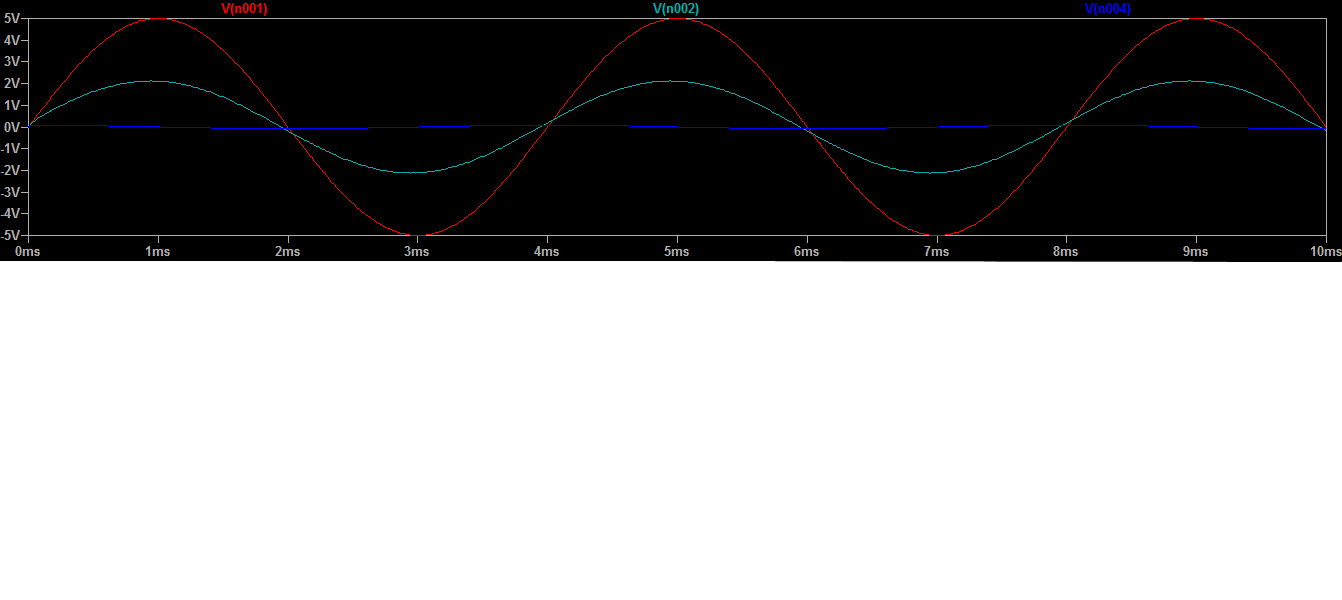
\includegraphics[width=\linewidth]{250hz.png}
  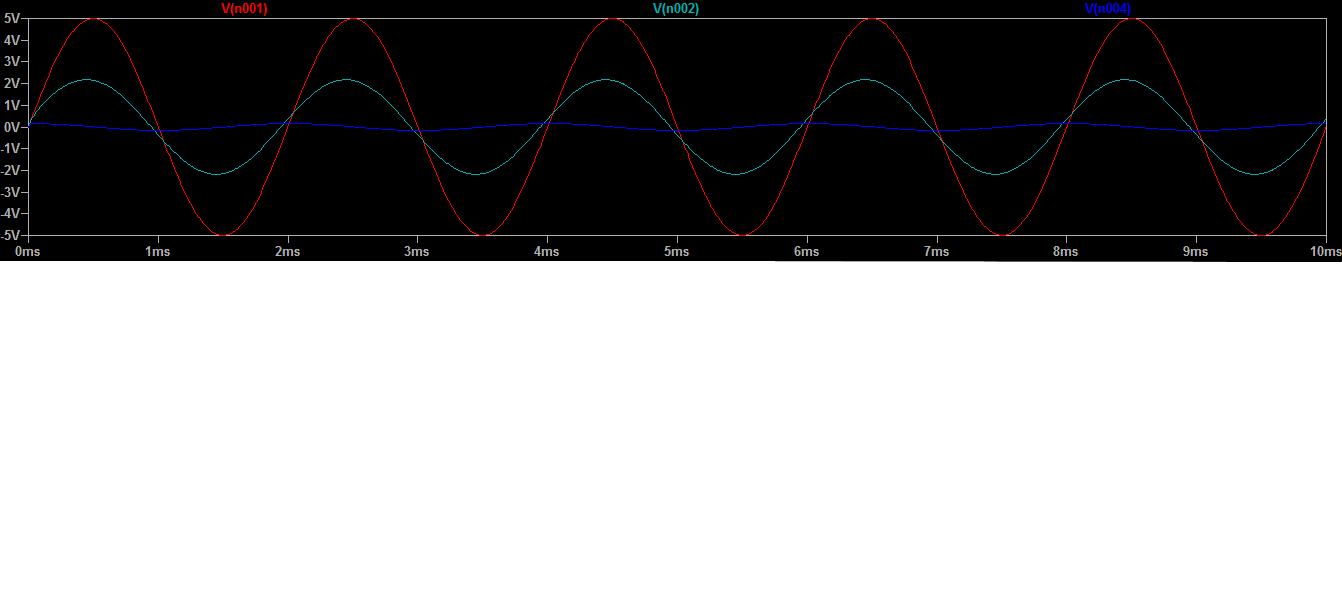
\includegraphics[width=\linewidth]{500hz.png}
  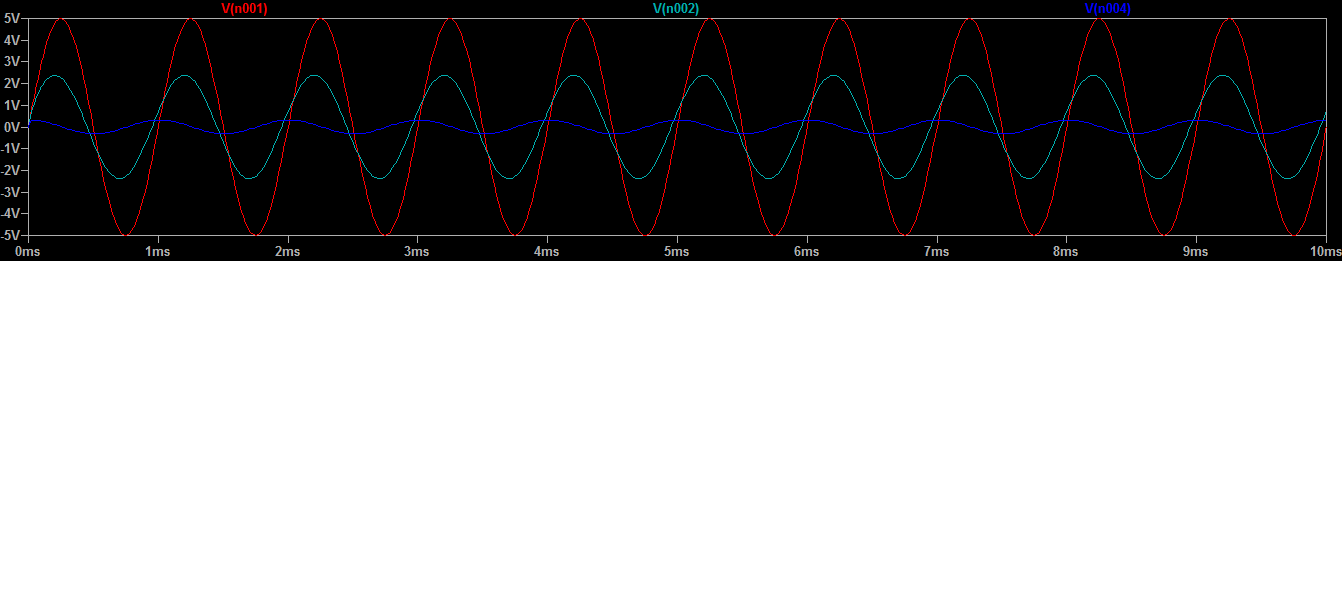
\includegraphics[width=\linewidth]{1khz.png}
  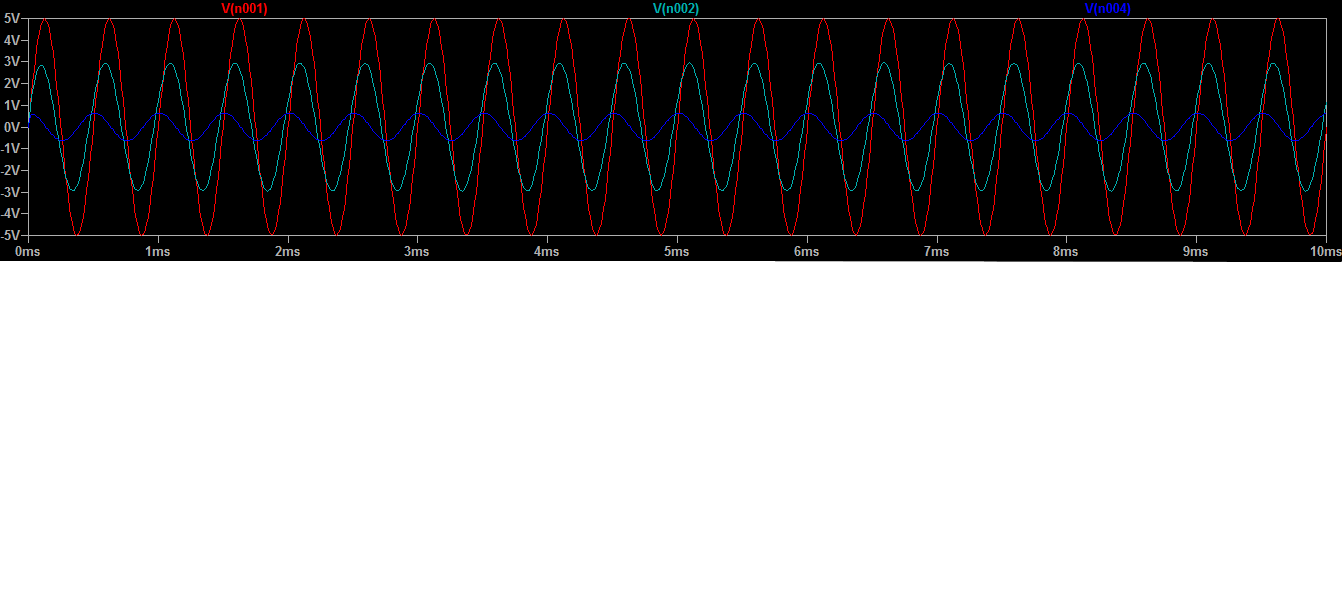
\includegraphics[width=\linewidth]{2000hz.png}
  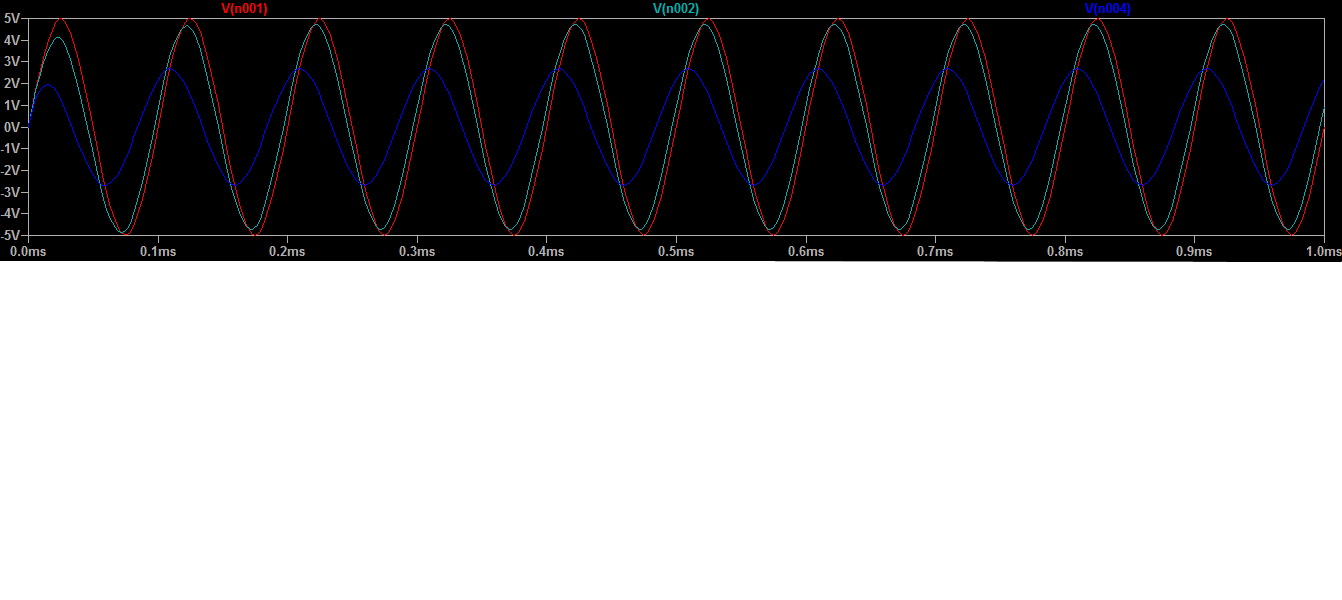
\includegraphics[width=\linewidth]{10000hz.png}
\end{figure}

%END KYLE

\end{document}
